\documentclass[11pt,a4paper]{article}
\usepackage[top=50pt,bottom=40pt,left=60pt,right=50pt]{geometry}
\usepackage[utf8]{inputenc}
\usepackage{amsmath}
\usepackage{amsfonts}
\usepackage{amssymb}
\usepackage{rotating}
\usepackage{verbatim}
\usepackage{graphicx}
\usepackage{hyperref}

\author{Judith van Stegeren and Mirjam van Nahmen}
\title{Development of the Mars Rover robot}

\begin{document}

\maketitle

%FirstPart:
 
% Description of the work on the Mars Rover
%   Describe the details of the main development activities:
\section{Introduction}
The main goal of this project is to build a Mars Rover robot that can autonomously find all lakes in the vicinity and measure the temperature in each of them.

% Listing of requirements with priorities.
\section{Requirements}
\begin{tabular}{|p{5cm}|p{10cm}|} 
\hline
MoSCoW & requirement\\
\hline
\hline
  \textbf{Functional requirements} & The robot must be able to ...\\
\hline
M & find all lakes.\\
%M & find a lake and determine its color.\\
%M & navigate around lakes.\\
M & avoid falling off the table.\\
M & notice obstacles in the area and avoid them.\\
M & measure the temperature of all lakes.\\
%M & see the difference between black, white, red, green and blue.\\
S & recognize bumping against an obstacles and drive around it.\\
S & when finished, show an overview of the collected data.\\
\hline

  \textbf{Usability} & The robot must ...\\
\hline
M & be programmed by stating its behavior in a DSL and then generating code from that specification.\\
M & stop when the robot is finished.\\
S & provide feedback for the user about measurements it makes.\\
C & not drive faster than 0,20 m/s, so that if the robot is heading for the edge of the table, the user still has time to interfere.\\
%S & provide feedback for the user about the state of the program for debugging purposes.\\
%M & provide feedback for the user when the robot is finished and the user press a button.\\
C & provide feedback for the user about errors/bugs.\\
\hline

  \textbf{Reliability}& \\
\hline
%M & The robot components must be tested before it will work with the whole system.\\
M & The program of the robot must not consume too much memory.\\
C & The robot must stop the motors whenever an error is detected.\\
S & The sensors must be calibrated before the program starts.\\
%The robot must have enough power and memory to run the programs.\\
%C & The robot must recognize its starting position.\\
\hline

  \textbf{Performance}&\\
\hline
M & If the light sensors spot the white border, the robot must react immediately.\\
S & If the light sensors spot the color border of a lake, the robot must react immediately.\\
S & The robot should not measure the same lake twice.\\
C & The robot should be able to find all lakes in 10 minutes. \\

\hline
   \textbf{Supportability}&\\
\hline
W & The DSL can also be used for the generation of code in another language or for use with a different API.\\
\hline
\end{tabular}

\pagebreak 
% Deployment with distribution of sensors, actuators and software components over NXT bricks; give both the own proposal and the chosen deployment, including motivation.
\section{Deployment}
\subsection{Our proposal for deployment}
List of the actuators:
\begin{itemize}
\item 2 motors
\item 1 motor for  the temperature sensor
\item 1 lamp
\end{itemize}

\noindent List of the sensors:
\begin{itemize}
\item 1 temperature sensor
\item 2 light sensors
\item 1 color sensor
\item 1 ultra sonar
\item 2 touch sensors
\end{itemize}

There can be 3 actuators and 4 sensors on 1 brick.
Since it is vital that the motor does not fall off the table, we want that the communication between the light sensors and the motors happens without Bluetooth. Since collision with other objects is an important issue, it would seem logical to connect the touch sensors directly with the master brick as well.\\ 

Since the color sensor, the motor for the temperature sensor and the temperature sensor all have to do with the same functionality, it would seem logical to put these sensors and actuators on the same brick. Finally, as the measurement of the distance with the ultrasonic sensor is not crucial for the functionality of the robot, we suggest to put that sensor on the (slave) brick for the measurements as well.\\

\textbf{Deployment diagram}\\
\begin{tabular}{|p{3cm}|p{6cm}|p{6cm}|} 
\hline
\textbf{brick} & \textbf{NXT1 (master)} & \textbf{NXT2 (slave)}\\
\hline
tasks & wandering, navigating, avoiding collisions & recognizing colors, spotting far-away objects, temperature sensor control, lamp\\\hline
actuators & motor 1, motor 2 & temperature sensor motor\\\hline
sensors & light sensor 1, light sensor 2, touch sensor 1, touch sensor 2 & ultra sonic sensor, temperature sensor, color sensor\\
\hline
\end{tabular}

\subsection{Use cases}
\begin{description}
\item[Wandering within white line] The robot drives in a straight line until it encounters a white line with one of its light sensors. If it encounters the white line, it will back up a bit, make a turn away from the white line and proceed in a straight line. For this use case, we need both motors and both the light sensors.
\item[New lake detection and measurements] On detection of a colored lake, the robot first checks if it hasn't encountered the lake before. If not, the robot positions itself before the lake. It then lowers the temperature sensor, measures the temperature and stores it together with the color of the lake. We need the color detector, the motor for the temperature sensor and the temperature sensor itself.
\item[Old lake detection] On detection of a colored lake, the robot checks if he encountered this lake before. If this is the case, the robot drives around the lake. For this we need the color detector and the two motors, but it doesn't matter whether the color sensor is on the same brick as both motors.
\item[Wandering without collisions] The robot drives in a straight line. If one of the bumpers touches an object, the robot backs up, makes a turn and proceeds in a straight line. For this we need the bumpers and both motors. Since reaction time is important in this use case, it would be best if the motors and the bumpers are connected to the same brick. The ultrasonic sensor can also play a role in this use case. The reaction time of the ultrasonic sensor is less important since it can spot obstacles from further away. %The touch sensors are for the situation that the sonar missed something, so it could be an advantage to put the sonar also on the brick of the motors. The communication with the sonar does not have to be instantaneous, so we could use Bluetooth, but it seems not the best thing to do.
\item[Ready] If the robot has measured the temperature in a lake, it check if all lakes have been measured. If that is the case, it stops wandering and shows the table with the temperatures of all lakes on his display.\\
\end{description}

\subsection{Actual deployment}

\begin{minipage}[t]{0.4\textwidth}

\textbf{Brick 1 (Master):} \\
crucial processes (wandering without \\collisions or falling off the table)

	\begin{tabular}{|c|l|}
	\hline
	A & Motor left\\
	B & Motor right\\
	C & Lamp yellow\\
	S1 & Light sensor left\\
	S2 & Light sensor right\\
	S3 & Touch sensor left\\
	S4 & Touch sensor right\\
	\hline
	\end{tabular}
	
\end{minipage}
\begin{minipage}[t]{0.2\textwidth}
	\begin{itemize}
	\item[ ]
	\end{itemize}
\end{minipage}
\begin{minipage}[t]{0.4\textwidth}

\textbf{Brick 2 (Slave):} \\
measurements (color of a lake, temperature and distance detection)

	\begin{tabular}{|c|l|}
	\hline
	A & Motor Temperature\\
	B & \\
	C & Lamp green\\
	S1 & Color sensor\\
	S2 & Ultrasonic sensor\\
	S3 & Temperature sensor\\
	S4 & \\
	\hline
	\end{tabular}
\end{minipage}

% Listing of the identified risks.
\section{Risk analysis}

\begin{tabular}{|p{0.4cm}|p{1.5cm}|p{3cm}|p{0.4cm}|p{0.4cm}|p{1.3cm}|p{3.5cm}|p{3.5cm}|} 
\hline
  Id & Type & Description & \rotatebox{90} {Probability} & \rotatebox{90} {Severity} & Weight & Mitigation & Contingency\\
\hline
\hline
 1 & Technical risk & The computer with the installed software breaks down and we lose access to our work. & 3 & 4 & High & Push all work to the repository, regularly. & Find a replacement for the broken laptop or use one of the lab computers.\\
\hline
 2 & Organiza- tional risk & The robot is not available for testing. & 3 & 4 & High & Regularly test small pieces of code, so that debugging is not a lot of work. & Postpone testing until later or wait until the robot is free. Use the lab when when we know there won't be other students around (early morning).\\
\hline
 3  & Technical risk & The DSL does not fit with the implementation. & 3 & 2 & Medium & Change the DSL to a lower level of abstraction. & \\
\hline
 4 & Organiza- tional risk & One of our team members become ill. & 3 & 2 & Small & Healthy living & The other one continues working on the project and the ill person works as much as possible from home. Keep communicating via email/chat.\\
\hline
 5 & Require- ments risk & The requirements contains ideas which are not compatible with the idea of the DSL. & 2 & 2 & Medium &  & Change requirements until it is possible to implement.\\
\hline
 6 & Technical risk & Problems with the Bluetooth communication between the two bricks & 5 & 3 & Medium & Test Bluetooth functionality as soon as possible. & Ask for help from the teacher or other students.\\
\hline
 7 & Organiza- tional risk & Lab partners have different schedules which makes it hard to find time to work together & 5 & 3 & Medium & The lab partners don't plan anything on Wednesday afternoon, so that there is at least one moment in the week when they are both free to work on the project & Reschedule work or work together during the weekends.\\
 \hline
\end{tabular}

\section{DSL}
\subsection{Approach}
We had two options for the structure of the DSL of the Mars Rover. 

Our first option was to create a DSL that was close to the subsumption architecture as implemented by the LeJOS API. The advantage of this approach is that we already had experience with programming in terms of behaviors during the first weeks of the Mars Rover project. It would also mean that we didn't have to worry about implementing an Arbitrator, as it would be provided by LeJOS. 
However, since the use of an arbitrator means that you sacrifice transparency for convenience, we did also foresee some problems with programming and debugging: the arbitrator would be an extra layer between us and the robot. 
%However, we found that the subsumption architecture was not general enough.
% The advantage of this approach is the experience with during the last weeks of the class 'Design of embedded Systems' and the Thread/task management is already made in form of the Arbitrator class.\\

The second option is the implementation of a state machine.
%approach which was the first idea for our DSL. 
In this case, the advantage of a state machine implementation is the great level of abstraction that we can use for the DSL. 
It's quite easy to design a robot by simply drawing an automata with the desired behavior.

%We see the advantages here in the abstraction level which can be create. 
%That makes it easier for us to implement such complex things like the Bluetooth communication, where we had a lot of problems with the Arbitrator. 
A disadvantage is the implementation of the state machine framework. 
We would have to implement this framework ourselves, which meant that instead of having a ready-made environment for programming, we would need more start up time for the project. However, we kept this in mind when we made the planning.
%It turned out to be no problem at all, since we could program very fast when eventually the state machine implementation was up and running.
%We do not have many experience with it, such that it will be approximately cost more time to implement the robot.\\

After some deliberation, we have chosen the state machine approach.
Firstly, this was because of the possibility to have more control over the Threads and tasks of the robot. 
We would have a better overview about what the robot does and why. 
Another reason is that the state machine approach is also more abstract, which suits the use of a DSL. 
Because of the high level of abstraction it is easier to make the implementation modular. 
From a commercial point of view, another advantage is that this way our implementation is reusable for comparable projects. 
%That is in the future useful to use it again for comparable projects which is in the business world quite often the case.  
And finally, it seemed to us that this approach was the most interesting to implement, with all its challenges.


\subsection{Syntax} 
%  Describe the concrete syntax of the DSL; what is the main idea, what is the meaning of the language?
The idea behind the DSL is a finite state machine. 
%In practice it is an often used concept from theoretical computer science.
%which uses states and arrows to describe the transitions and conditions in which the robot can be. 
A finite state machine, or automata, is a model of computation that can be in one of a finite number of states. It can change from one state to another by a transition or arrow.

A complete program for the Mars Rover robot is written in two instances of the DSL. Since we work with two bricks, we have an automaton for each brick: one for the master and one for the slave.

We start out by giving the automaton a name and a class. In the class we specify whether it is the slave or the master brick. We need to make this distinction for the code generation phase, since the master and slave have very different actuators and sensors and thus a different set of permissible actions.

\begin{verbatim}
Automaton: bumpercarexample
        Class: master
\end{verbatim}

Then we list all states of the automaton. 
We signify the start of this list by the keyword \texttt{States:}, and the definition of a state starts with the keyword \texttt{State}.
Each state has a name and a (possibly empty) list of actions. 
Whenever the robot enters in state $s$, all actions of $s$ will be executed in the specified order.

\begin{verbatim}
States: 
        State start             do drive forwards INF speed 200
        State problemLeft       do stop, turn right (15,90)
        State problemRight      do stop, turn left (15,90)
        State finished          do stop
\end{verbatim}

In this example, whenever the robot is in state \texttt{start}, it starts the motors to drive forwards. In \texttt{problemLeft} and \texttt{problemRight}, it stops the motors and makes a turn. In the state \texttt{finished} it stops the motors.

Finally, we have to specify the transitions of the automaton, ie. when we can move from one state to the other. We make another list \texttt{Arrows:}, where we specify the transitions. Note that the order in which we define the transitions from $a \rightarrow b$ is relevant for the order in which we check the possible transitions in the method for state $a$.

Each arrow consists of three parts: two states (the origin and destination of the transition) and a condition. When we are in a state $s$ that has a transition to $s'$, we are only allowed to change to $s'$ if the matching condition is fulfilled. 

The syntax for the specification of a transition is
\[ \texttt{Arrow origin -> destination	if condition} \]
where condition is a list of conditions in disjunctive normal form. 
Disjunctive normal form means that a boolean formula consists of disjunctions of conjunctive clauses. The conjunctive clauses are placed between brackets and prefixed with the keyword \texttt{and}.
Since every boolean formula has a disjunctive normal form, we thought it was a cool solution for more complex conditionals without having to implement boolean operators completely from scratch. In practice we hardly used complex conditionals, so in the end it also meant more typing work for the programmers.

\begin{verbatim}
Arrows: 
    Arrow start -> problemLeft          if (and lightsensor left reads white) 
                                           (and bumper left is pressed)
    Arrow problemLeft -> start          if (and lightsensor left reads black 
                                                bumper left is not pressed)
    Arrow problemLeft -> problemLeft    if (and lightsensor left reads white) 
                                           (and bumper left is pressed)
    Arrow start -> problemRight         if (and lightsensor right reads white) 
                                           (and bumper right is pressed)
    Arrow problemRight -> problemRight  if (and lightsensor right reads white) 
                                           (and bumper right is pressed)
    Arrow problemRight -> start         if (and lightsensor right reads black 
                                                bumper right is not pressed)
    Arrow start -> finished             if (and timeout 10 sec)

\end{verbatim}

In the first arrow of our example, we have a conditional that consists of two single-element-clauses. This means that we can go from \texttt{start} to \texttt{problemLeft} if
\[ \texttt{lightsensor reads white} \vee \texttt{bumper left is pressed} \]
The second arrow consists of only one clause, which we can read as follows:
\[ \texttt{ lightsensor reads black} \wedge \texttt{bumper left is not pressed} \]

Finally, we need to define a starting state and a set of final states:
\begin{verbatim}
    Start state: start 
    End state: finished
\end{verbatim}
Whenever the program is started, the start state is the state where we begin. 
If we during execution of the program end up in a final state, we execute the actions of the final state and then stop taking transitions, ie. the program is finished.

\subsection{Actions and conditions}
We have tried to reflect the actuators/sensor division in the state machine framework. We have tried to incorporate the actuators of the robot in the actions of the DSL, and the sensor input in the conditions for the transitions.

\subsubsection{Actions}
\begin{tabular}{p{6cm}p{10cm}}
\textbf{example syntax} & \textbf{description}\\
drive \emph{\{forwards,backwards\}} duration \emph{\{duration,INF\}} speed \emph{speed} & Robot drives in \emph{direction} with speed \emph{speed}. Motor keeps running for \emph{duration} or indefinitely.\\
turn (\emph{min},\emph{max}) & Robot makes a turn with random angle between \emph{min} and \emph{max}.\\
stop & Both motors immediately stop.\\
send \emph{message} & The robot sends package with \emph{message} to the other brick.\\
park & The robot tries to maneuver in such a way that it is aligned with a lake, as necessary for doing a temperature measurement.\\
init bt \emph{slave}& Initalizes a Bluetooth connection with \emph{slave}\\
wait for bt & Wait for a Bluetooth connection from another brick\\
calibrate & The robot asks the user to place it on the white and black parts of the robotics area, and tries to save the sensor values of the left light sensor. Must be called in the starting state for proper functioning.\\
beep & Robot emits a beeping sound.\\
print \emph{string} & Robot prints \emph{string} on the screen.\\
consume package & Robot consumes one message from the message queue, does nothing if the queue is empty.\\
consume sonar package & Robot consumes sonar messages from the message queue until the queue is empty or the first package is not a sonar package.\\
temparm \emph{\{up,down\}} & arm for the temperature sensor goes up/down\\
temparm measure & Robot performs a measurement with the temperature sensor.\\
\end{tabular}

\subsubsection{Conditions}
\begin{tabular}{p{6cm}p{10cm}}
true & Always true, is used for transitions without condition\\
receive \emph{message} & true if the head of the message queue contains a package with \emph{message}\\
lightsensor \emph{\{left, right\}} reads \emph{\{black, white\}} & true if the lightsensor on the specified side reads the specified value.\\
colorsensor reads \emph{color} & true if the colorsensor reads \emph{color}\\
color is new & true if the color that the colorsensor found last has not been checked\\
sonar detects \emph{\{something, nothing\}} at \emph{distance} & true if the sonar detects an object closer than \emph{distance}\\
bumper \emph{\{left, right\}} is \emph{\{pressed, not pressed\}} & true if the bumper on the specified side is (not) pressed.\\
timeout \emph{time} \emph{\{ms,sec\}} & true if the robot has been in this state for longer than \emph{time} \emph{unit}.\\
all colors found & true if all lakes in the measurement array are flagged as 'found'\\
\end{tabular}
%What we did NOT implement, but would have done if we had more time:
%formally restrict the actions one can do as a slave or master (ie. in the DSL).

\subsection*{Instances for the Mars Rover}
%  Describe the instance(s) of the DSL that are used for the Mars Rover, explain the main idea.
We have made 20+ instances during the development of the Mars Rover. We will elaborate only on the instances used for the final program.
We use one instance for every brick.

Since we use a state machine, we wanted the following assumptions to hold when designing the automatons:
\begin{enumerate}
\item every state is a black box without weird side effects, ie. when the current state is not s1, no part of s1 will be executed.
\item the outgoing arrows of every state should together cover all possible situations. If not, we can get stuck in one of the states.
\end{enumerate}

The instances we have defined for the master and slave bricks are a description of the following automatons:

\subsubsection{Master}
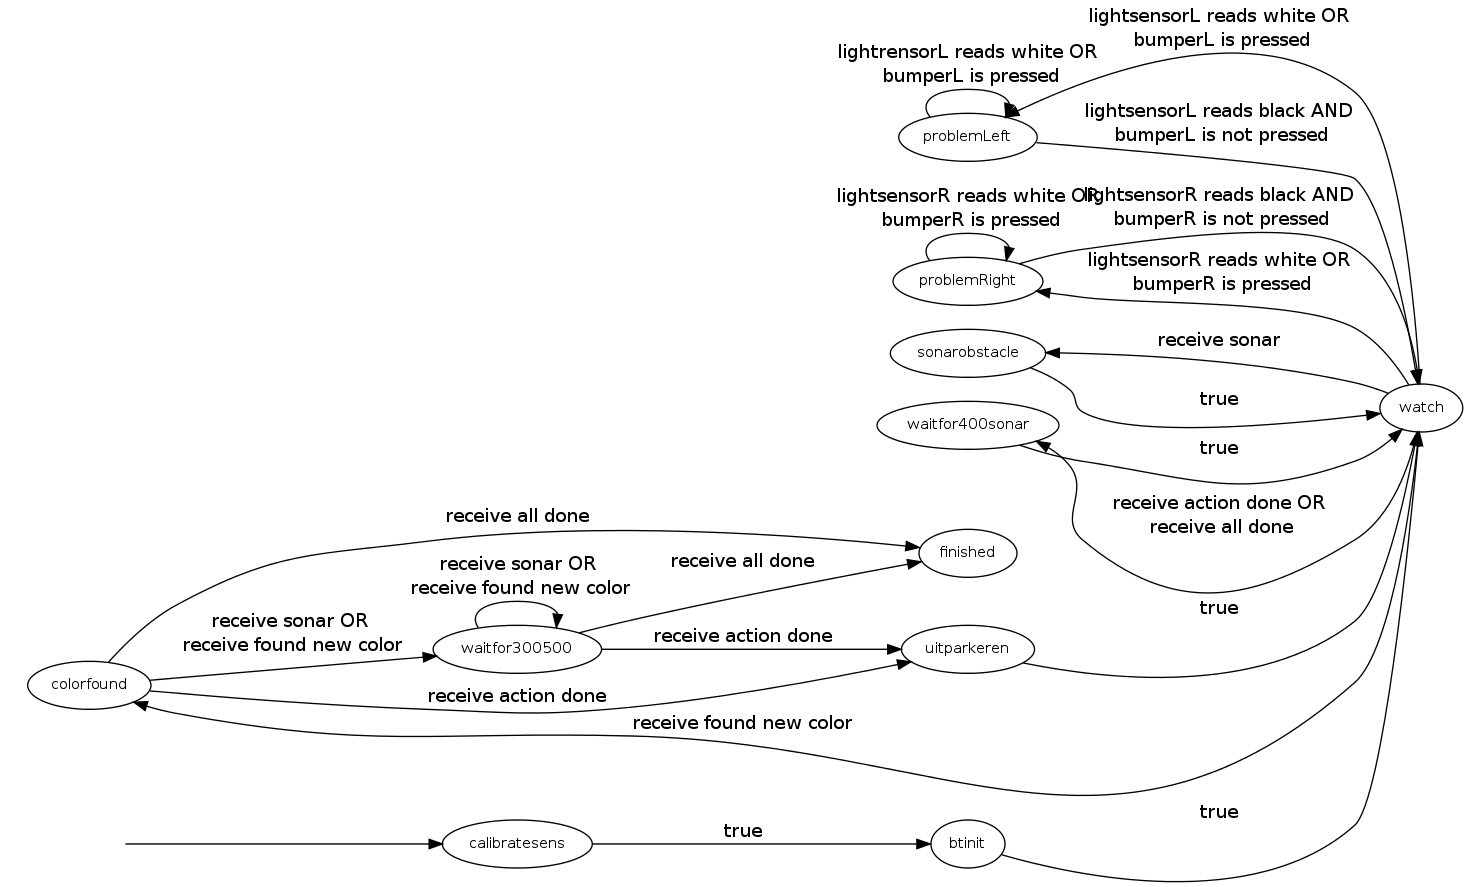
\includegraphics[width=24cm,angle=90,origin=c]{t9-m.png}

\subsubsection{Slave}
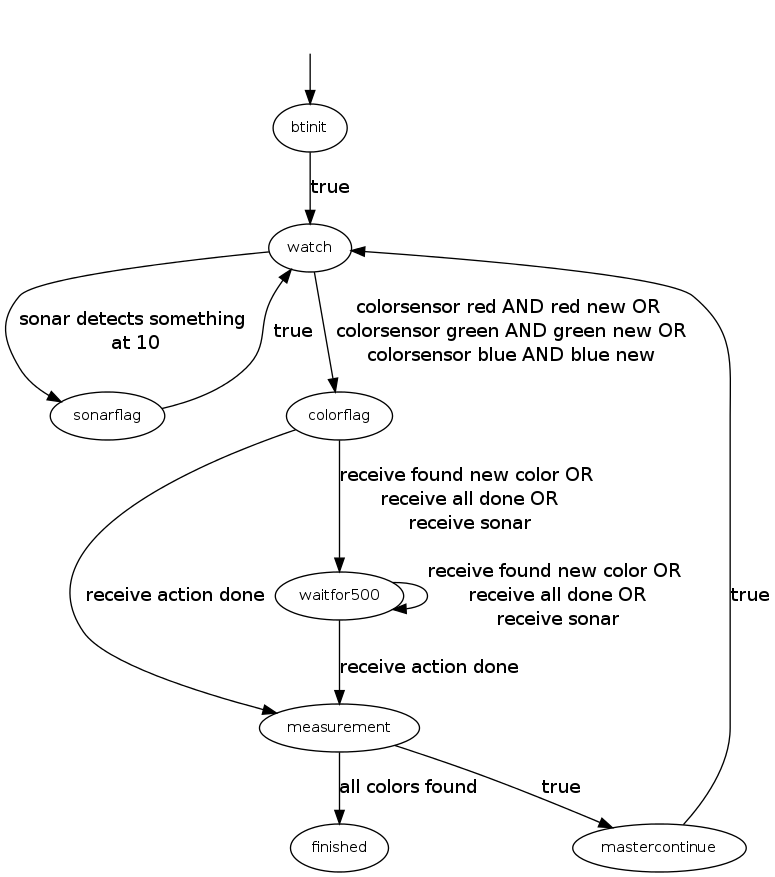
\includegraphics[width=16cm]{t9-s.png}

\subsection{Main structure of the generated code}
% Describe the main structure of the generated code.
%- slave /Master unterschiede
%- actions / condition use
%- states in enum / methods created
The Main classes for the slave and for the master are be generated of the two instances. Every main get  own equipment so that the ports and used variables can be declared and initialized. \\
In the \emph{JavaGenerator.java} is this solved with the \emph{masterEquipment(), slaveEquipment(), masterInit(), slaveInit()} to decide which allocation should be generated in the Main classes for the slave and for the master. To handle the states from the automaton will be an enum generated which contains all states, such an enum of the mars rover looks like: 
\begin{verbatim}
public enum State {
    CALIBRATESENS,
    BTINIT,
    SONAROBSTACLE,
    COLORFOUND,
    WAITFOR300500,
    WAITFOR400SONAR,
    UITPARKEREN,
    FINISHED,
    WATCH,
    PROBLEMLEFT,
    PROBLEMRIGHT
}
\end{verbatim}

The public variable \emph{current} will be used to keep the current state. Every state has also his own method where all the actions of this state will be executed. After all actions are done the state waits for the next trigger which indicates the next transaction and the next state becomes the current state. 
The method \emph{execute(State s)} connects the enum with the methods of a state. Also the start and end state are be defined in this way. \\
The arrows of the automaton contains the conditions of an transition. These conditions are checked during the while the automaton waits for the trigger for the next state. Every condition is written as an if-statement with the next state as body. \\

The most difficult part of the program was the integration of Bluetooth, we decided to created a new Thread for the read part of the communication. For this the master and the slave use both the class \emph{BTfunctionality}, which contains the information for the Bluetooth part. Further is the master also the master of the Bluetooth communication and initialized also the handshake and the set up of the connection. \\

The found lakes and the corresponding information are saved in the array lakes of the object Lake. So that it is in every situation possible that the slave can edit the array. \\

For debugging and readability reasons we also created the Thread \emph{Colorfunctionality} which shows in every situation the actual found color in the display of the slave.  
  



\section{Realization of the Mars Rover}
% Describe the order in which features of the Mars Rover have been implemented.
\subsection{Approach}
The first steps were to design and implement the basic structure of the DSL and the code generation. We decided to use the state diagram and designed the start/end state and the robot should be able to wander an area without falling off the table. 

We built the rover by incrementally implementing the concepts we needed for the rover. Our first goal was to have a rover that could drive around freely without falling off the table. It took us more time to implement this basic functionality than normal, since we had to implement the state machine framework before we could test our instances of the DSL!
After two weeks we had a working framework and a first stub of a DSL. 

At the beginning, we have made a list of elements of the project where we anticipated problems with the implementation: 
\begin{itemize}
\item Bluetooth communication and working with Threads
\item communication protocol / packets between the two bricks
\item usage of the RCX motor and temperature sensor
\item code generation -- we wanted the code to be clear and modular
\item maneuvering around the lakes ("parking"), in such a way that the temperature sensor finishes in the right position.
\item color recognition in different lighting conditions
\end{itemize}

To mitigate these potential problems, we decided to build small test instances for every problem before incorporating new functionality in the final program. Because of this incremental, modular approach, every problem could be spotted and debugged in an isolated test case, which made everything easier. The test instances can be found in the git repository (\url{https://github.com/jd7h/des/tree/master/eindopdracht/DSL/test}). 

\subsection{Planning}
Every week during the project, we would do the following:
\begin{enumerate}
\item Choose a problem to tackle
\item Describe a set of automatons with the desired functionality (small test cases and a bigger test which incorporates new and old functionality)
\item Expand the DSL until the automatons can be described in the DSL
\item Expand the code generation files until the instances generate valid code.
\item Test all instances, starting with the small test cases and revise the DSL and/or code generator until everything works properly. 
\end{enumerate}

\begin{tabular}{|r|p{10cm}|}
\hline
week & problems tackled\\
\hline
December 1	& state machine framework \& wandering without falling off the table\\
December 2	& state machine framework \& wandering without falling off the table\\
December 3	& Bluetooth, calibration of sensors, communication, basic functionality\\
December 4	& communication between bricks\\\hline
January 1	& communication and package handling, colorsensor, temperature sensor\\
January 2	& parking, testing the mars rover as a whole\\
\hline
\end{tabular}


%\subsection*{Final result}
% Describe the final result: what has been implemented exactly, which requirements are satisfied, which requirements are not satisfied and explain why not. 

%Second Part:
 % Evaluation of the work on the Mars Rover
 % Evaluate the work done and mention own observations. 
  % A list of relevant questions:
	% • What were the most important steps during the development; what was difficult, what
	%was easy, was the order of the steps suitable?
	% • How often did you change the DSL, is there a large difference with the DSL for the
	%small Lego NXT Rover, what where the reasons for changes?
	% • Looking back at your DSL and code generation; what would you do differently, what
	%could be improved (e.g., if you would have more time)?
	% • How flexible and extendable is your solution? For instance, how easy is it to add
	%sensors, actuators, to move them to another NXT brick, or to add new functionality?
	% • Evaluate the development process. Especially, discuss the use of a DSL for modeling
	%and code generation. What are advantages and disadvantages, what was difficult, what was easy?
	% • What are the observations about the technology used, such as Eclipse, LeJOS, Xtext,and Xtend?
	% • What are general lessons learned? 

\section{Evaluation of the work on the Mars Rover}
\textbf{What were the most important steps during the development; what was difficult, what was easy, was the order of the steps suitable?}\\
The most important steps of our Mars Rover project were in the beginning the decision to create a DSL in form of a state machine. With this decision we solved some problems we encountered during the project of the small Rover. For example the problem of the untransparent workings of the Arbitrator and the Bluetooth communication using a Thread. Because we used a deterministic automata approach, we knew in every state exactly what the robot does. The behavior of the robot was for us now more transparent, and this made the programming and working with the robot more easy. 
The decision created also some problems. We had to begin with building the framework from scratch and couldn't use much code from the small Rover. This was a challenge for us, because we had not much experience with LeJos and NXT without the subsumption architecture.

%\subsection{Planning}
We tried to work every week one day together in the DES-lab, but we had of course some problems. Because we both had very different schedules, it was hard to find time to work together. We managed to create a good task allocation and we could also work on different days. We also discussed every week a goal which should been reached, so that we could show a result to Jozef. As an effect of this is that we didn't stay to long on one complex problem and to find sometimes a solution which is more convenient and for that moment useful, but not really nice. %example?\\

To get the project more structured we made a list with subject which can be problematic and which need more time to find a good solution. This helped because we got early an impression how big the project becomes and we had in the beginning time to get in the subjects. A second advantage of this approach was that we could build our DSL around the difficult subjects and we didn't had to change the DSL so much. \\
During the whole programming phase we build small tests which are successive such that we could very nicely test every component separately. Further could we built the test that go more and more to a complete solution for the Mars Rover.\\

\textbf{Looking back at your DSL and code generation; what would you do differently, what could be improved (e.g., if you would have more time)?}\\
Because of the limited time of the project and the very narrow goal of the DSL -- the DSL is for only one mission and for only one robot (in our case, two robots, master and slave) -- the DSL is a bit less abstract than we would have liked. To complete the project in time, we had to focus on implemented the functionality that was most useful for the final demo. For this reason, we hardly have any code or grammar-specifications of things that we did not use heavily, such as the lamp and the sonar. 
We could also have spent less time on the Bluetooth implementation. We have a few problems with getting the Bluetooth communication to work during development, but since we did not exactly know the cause of the problem we spent a lot of time debugging. A tip from Jozef during the demo solved the issue, luckily, but it turned out to be a very minor thing and it should've taken less time.\\
If we had more time, we had changed and extended some different things. The Bluetooth works not perfectly with the ultra sonic sensor. The sensor sends non stop the distance to the master until he don't sees something, then he sends one time 500. But this blocks the other functions of the robot and it is possible that the robot goes always back until the sensor stops with sending. \\
A second thing is the calibration of the sensors, the robot is very addicted to the ambient light, a solution is to calibrate every light and color sensor before every start. At this moment the robot only calibrates the light values, this can be improved.\\

\textbf{How often did you change the DSL, is there a large difference with the DSL for the small Lego NXT Rover, what where the reasons for changes?}\\
Because of our test-driven approach, we extended the DSL weekly with new functionality. Since the DSL for the small rover was very limited, there is a big difference between the DSL for the small rover and the DSL for the mars rover. The small rover had no distinction between the master and the slave, there was only a limited set of actions and since we were still working with the subsumption architecture, we had to incorporate priorities in the DSL.\\

\textbf{How flexible and extendable is your solution? For instance, how easy is it to add sensors, actuators, to move them to another NXT brick, or to add new functionality?}\\
The fact that we use a state machine is useful in different ways. It makes it easy to create a model of the state machines. To change hardware components of the robot only the code generator has to be changed, that is positive, because the old instances of the robot can be reused. \\
For our robot is it also very easy to add some new functions. Our DSL is very structured and it is easy to add a new arrow with constraints and a new state with new actions in the instances. Also to add some new code is our code very good structured which makes it easy to add new functionality. \\
The Bluetooth 'protocol' we made is also extendable. We worked with a integers to identify the different messages, so it is easy to add new messages in the DSL. \\
The state machine approach was useful to structure the coding process, because we had to split every step of the robot in conditions for the arrow and actions which should be done when the conditions match. This made it also easy to split our tasks in basic stuff, condition stuff and action stuff. Also the way to solve a complex problem was in the way of thinking in which conditions are there and what should the robot do to reach the state we want. In the beginning we thought to big and to complex, but after the first few tests, we learned the advantages and it was easier to split the big problems in smaller ones which made it easier to solve it. \\

\textbf{Evaluate the development process. Especially, discuss the use of a DSL for modeling and code generation. What are advantages and disadvantages, what was difficult, what was easy?}\\
DSLs can have quite some advantages: the code from the codegenerator can be reused over and over, as it's easier to create new instances than to write an entire new program. It's nice and abstract and tailored to the problem at the same time, which means that people who are not programmers will have less trouble using a (well-designed) DSL than a programming language. 
We think the usage of a DSL to solve a set of problems is only useful if the developer is already familiar with the way a this particular set of problems has to be solved. Since the DSL has such a big impact in the code you can ultimately generate, the developer has to have a solution in his head before he can design the DSL. 
The design of the DSL is of course the hardest part, since this part completely determines everything you can do with it later on. We tackled this problem by looking directly at the (new) things we needed in the project. This way we were never 'stuck' and we never had to complete rewrite the DSL. The downside of this approach is that the DSL is a bit too specific for the mars rover mission.
The best way to design a DSL is trying to make the DSL as modular as possible, or at least design it in such a way that the codegenerator can work from the DSL in a modular way. It also allows you to extend or adapt the DSL in case the problem or the solution changes.\\

%\subsection{Eclipse, LeJOS, Xtext,and Xtend}
\textbf{What are the observations about the technology used, such as Eclipse, LeJOS, Xtext,and Xtend?}\\
Working with Java and NXT was new for us, but it worked very good. LeJOS, Xtext and Xtend are very well documented and also often used, so that there are many forums and blogs which answered to many of our questions we had during coding. Especially the API description is very good and explains many functions.\\
The only problem we had, is that the Java which is used for LeJOS does not support every basic functionality of Java. But to find this, we used a lot of try and error tests. \\

\textbf{What are general lessons learned?}\\
Working with hardware is not always deterministic because of the many influences outside of the system. It is also almost impossible to consider every possible situation what can be happen with the system. 

\end{document}
